\chapter{เอกสารสำคัญที่เกี่ยวข้อง}
\begin{itemize}
    \item \textbf{เอกสารสำคัญของคณะ}
          \begin{itemize}
              \item \hyperlink{target:approval}{หนังสือยินยอมให้เผยแพร่รายงานปฏิบัติงานสหกิจศึกษา} (หน้า \pageref{page:approval})
              \item \hyperlink{target:03-04}{วศ.สก.-03/04 รายงานตัวเข้าสหกิจศึกษา} (หน้า \pageref{page:03-04})
              \item \hyperlink{target:03}{วศ.ฝ.ค-03 แบบฟอร์มยืนยันการรับนักศึกษา} (หน้า \pageref{page:03})
              \item \hyperlink{target:06}{วศ.สก-06 แบบแจ้งโครงร่างรายงานการปฏิบัติงานสหกิจศึกษา} (หน้า \pageref{page:06})
              \item \hyperlink{target:10}{วศ.สก-10 แบบสรุปการปฏิบัติงานสหกิจศึกษาประจาสัปดาห์} (หน้า \pageref{page:10})
              \item \hyperlink{target:11}{วศ.สก.-11 แบบสรุปผลการปฏิบัติงานสหกิจศึกษา} (หน้า \pageref{page:11})
          \end{itemize}
    \item \textbf{เอกสารสำคัญที่เกี่ยวข้องกับงาน}
          \begin{itemize}
              \item \hyperlink{target:docker}{เอกสารสรุปสิ่งที่ได้เรียนรู้และลองทำ Docker} (หน้า \pageref{page:docker})
              \item \hyperlink{target:kube}{เอกสารสรุปสิ่งที่ได้เรียนรู้และลองทำ Kubernetes} (หน้า \pageref{page:kube})
              \item \hyperlink{target:jenkins}{เอกสารสรุปสิ่งที่ได้เรียนรู้และลองทำ Jenkins} (หน้า \pageref{page:jenkins})
              \item \hyperlink{target:terraform}{เอกสารสรุปสิ่งที่ได้เรียนรู้และลองทำ Terraform} (หน้า \pageref{page:terraform})
              \item \hyperlink{target:monitoring}{เอกสารสรุปสิ่งที่ได้เรียนรู้เกี่ยวกับ Monitoring Tools} (หน้า \pageref{page:monitoring})
              \item \hyperlink{target:elk}{เอกสารสรุปสิ่งที่ได้เรียนรู้เกี่ยวกับ ELK Stack} (หน้า \pageref{page:elk})
          \end{itemize}
\end{itemize}

% คณะ

\includepdf[pages=-, scale=.8, pagecommand={\hypertarget{target:approval}{},\label{page:approval}}, nup=1x1, frame=false]{pdf/approval}

\includepdf[pages=-, scale=.8, pagecommand={\hypertarget{target:03-04}{},\label{page:03-04}}, nup=1x1, frame=false]{pdf/03-04}
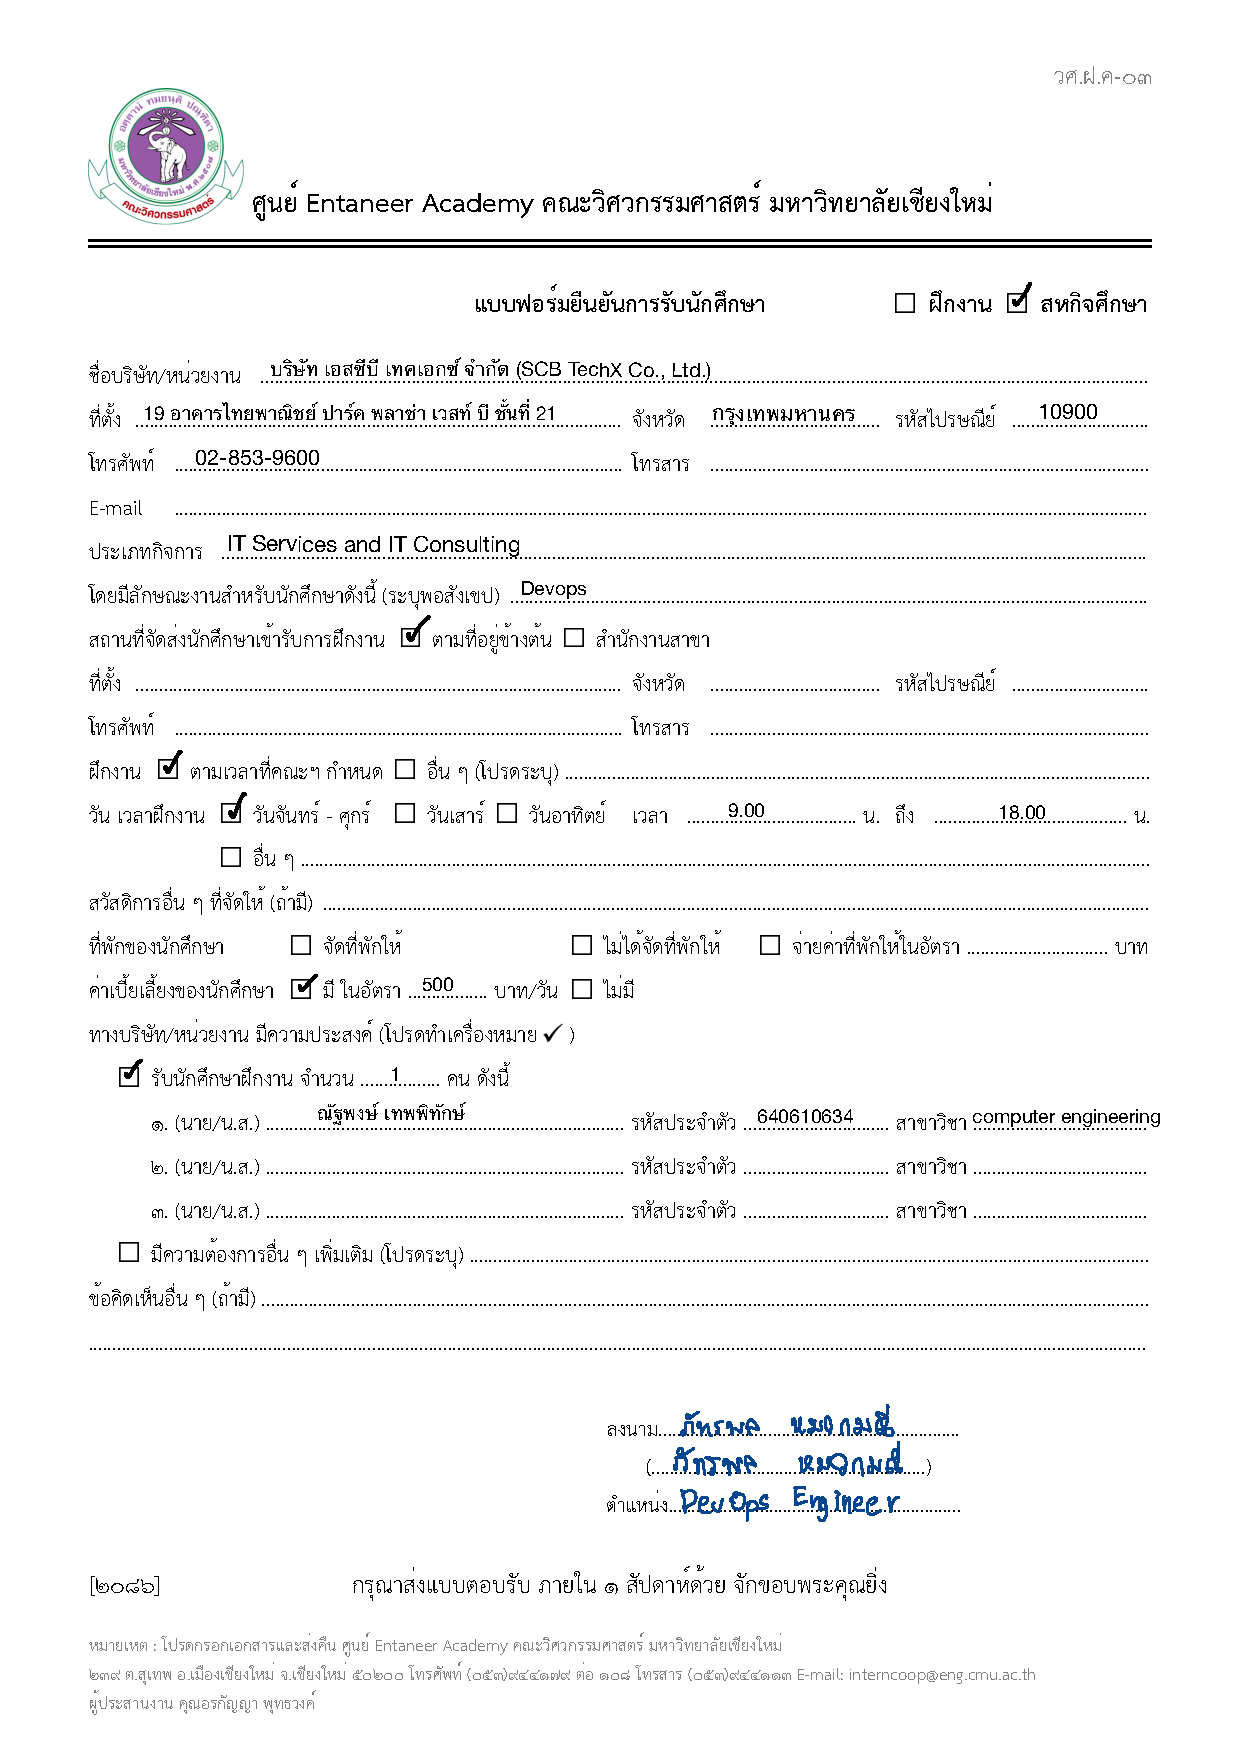
\includepdf[pages=-, scale=.8, pagecommand={\hypertarget{target:03}{},\label{page:03}}, nup=1x1, frame=false]{pdf/03}

\includepdf[pages=-, scale=.8, pagecommand={\hypertarget{target:06}{},\label{page:06}}, nup=1x1, frame=false]{pdf/06}
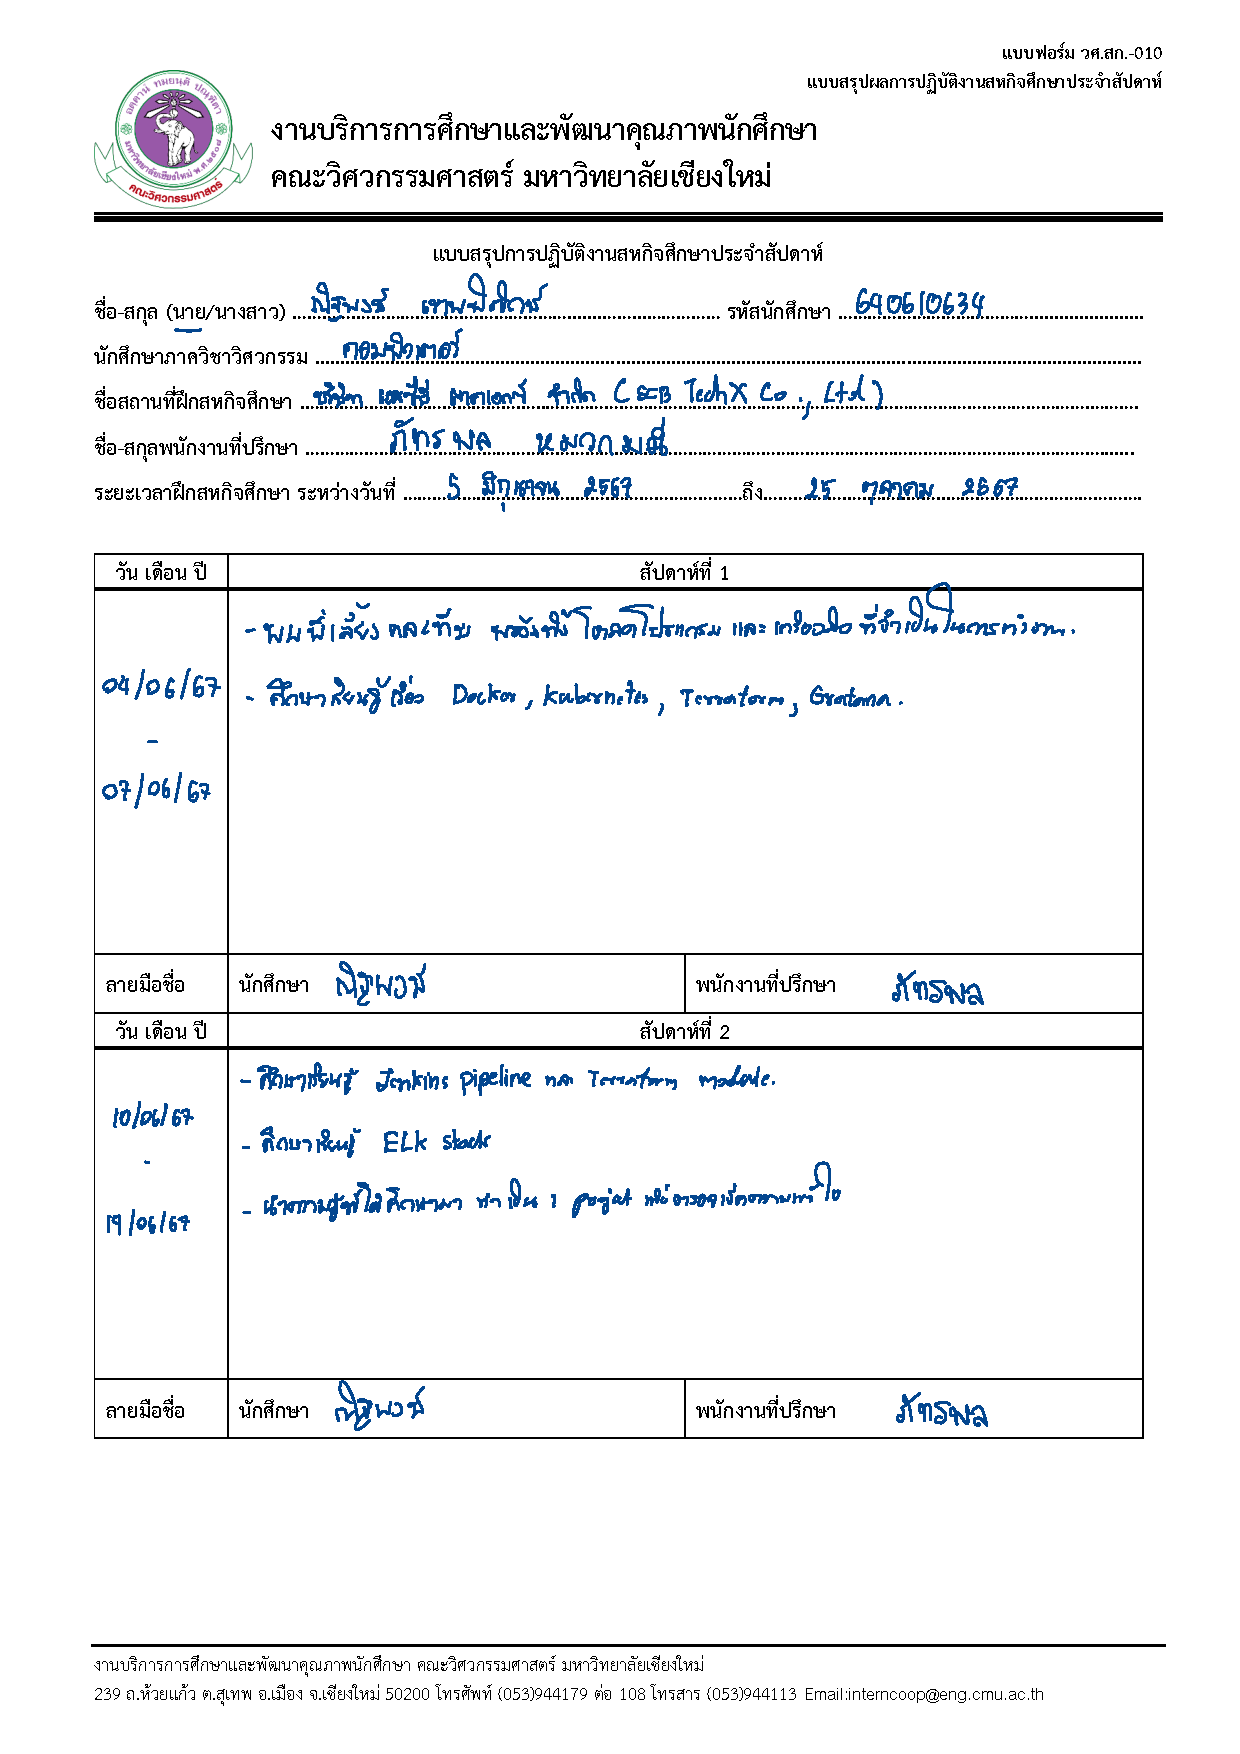
\includepdf[pages=-, scale=.8, pagecommand={\hypertarget{target:10}{},\label{page:10}}, nup=1x1, frame=false]{pdf/10}
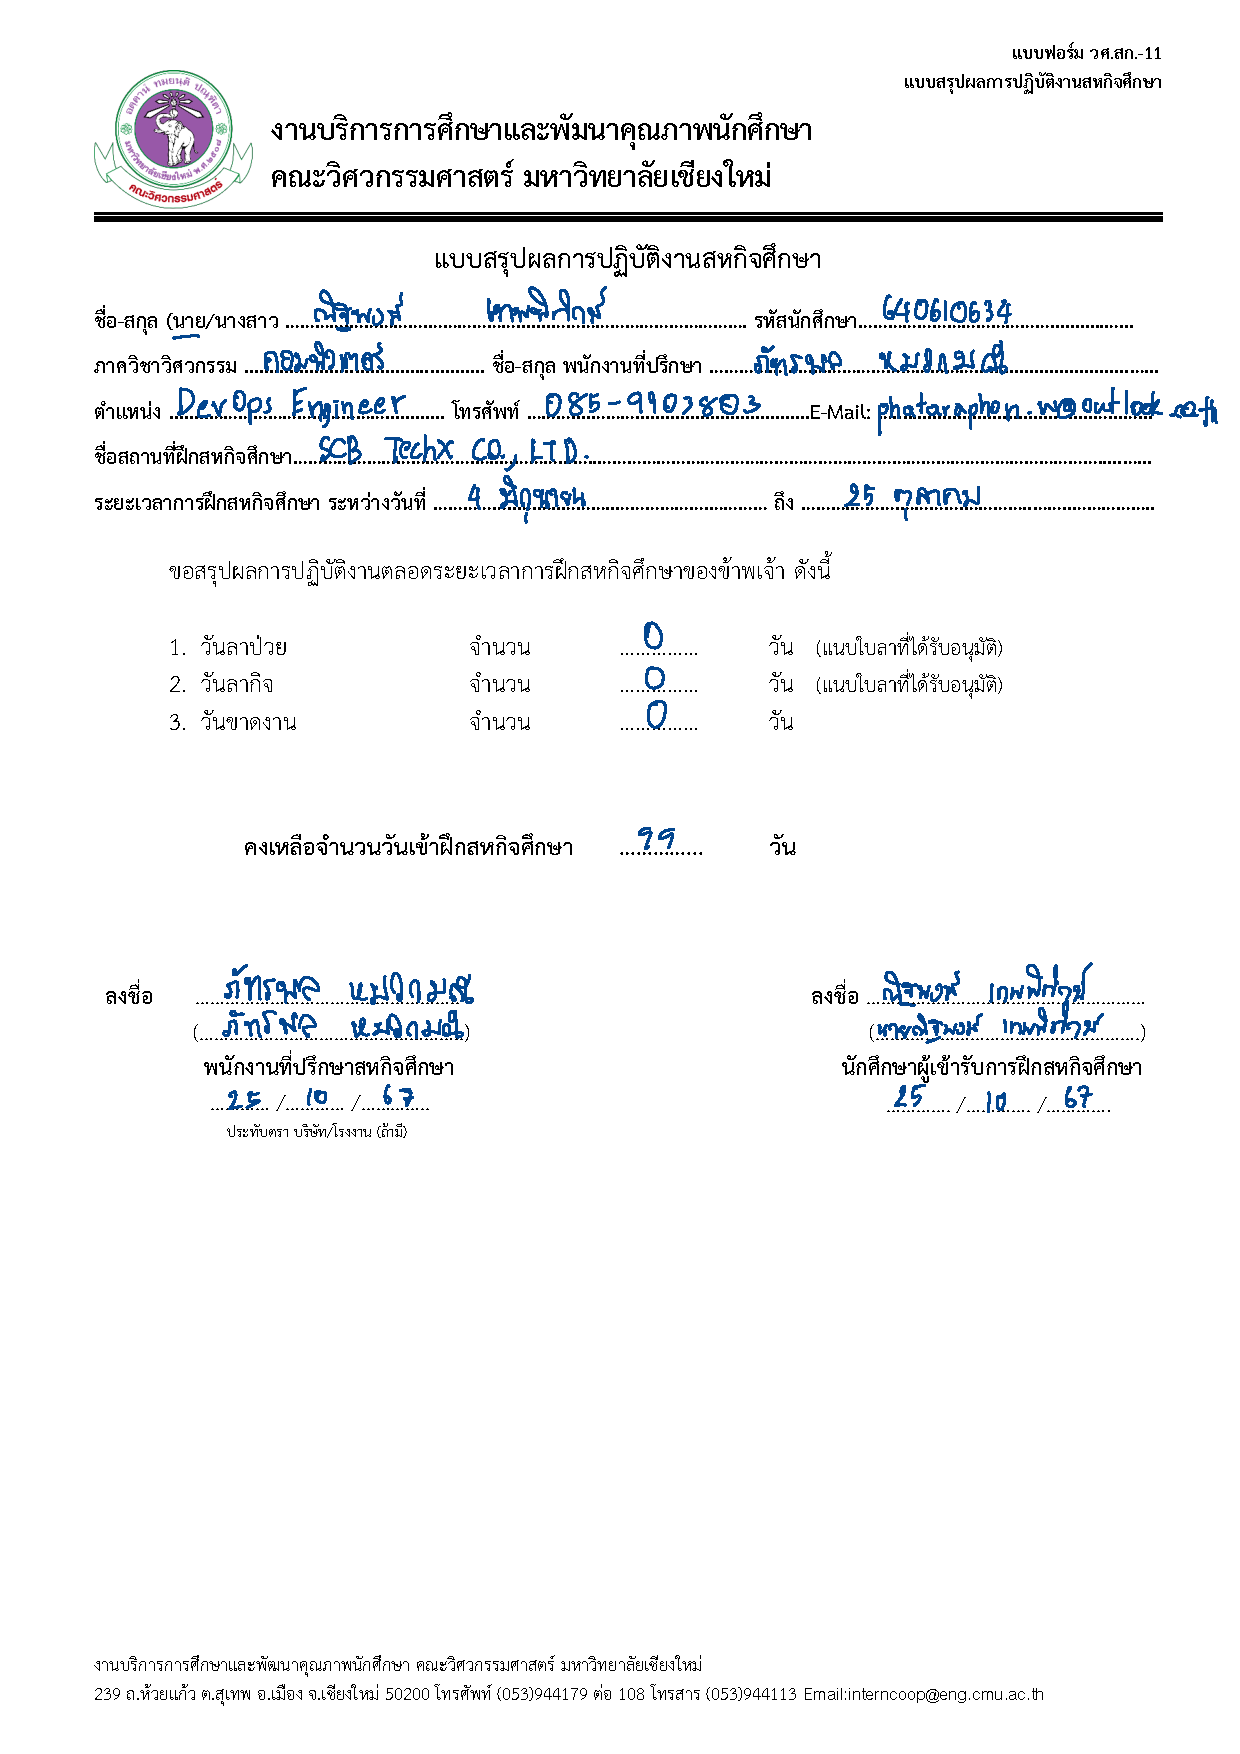
\includepdf[pages=-, scale=.8, pagecommand={\hypertarget{target:11}{},\label{page:11}}, nup=1x1, frame=false]{pdf/11}

% ส่วนที่เกี่ยวข้อง
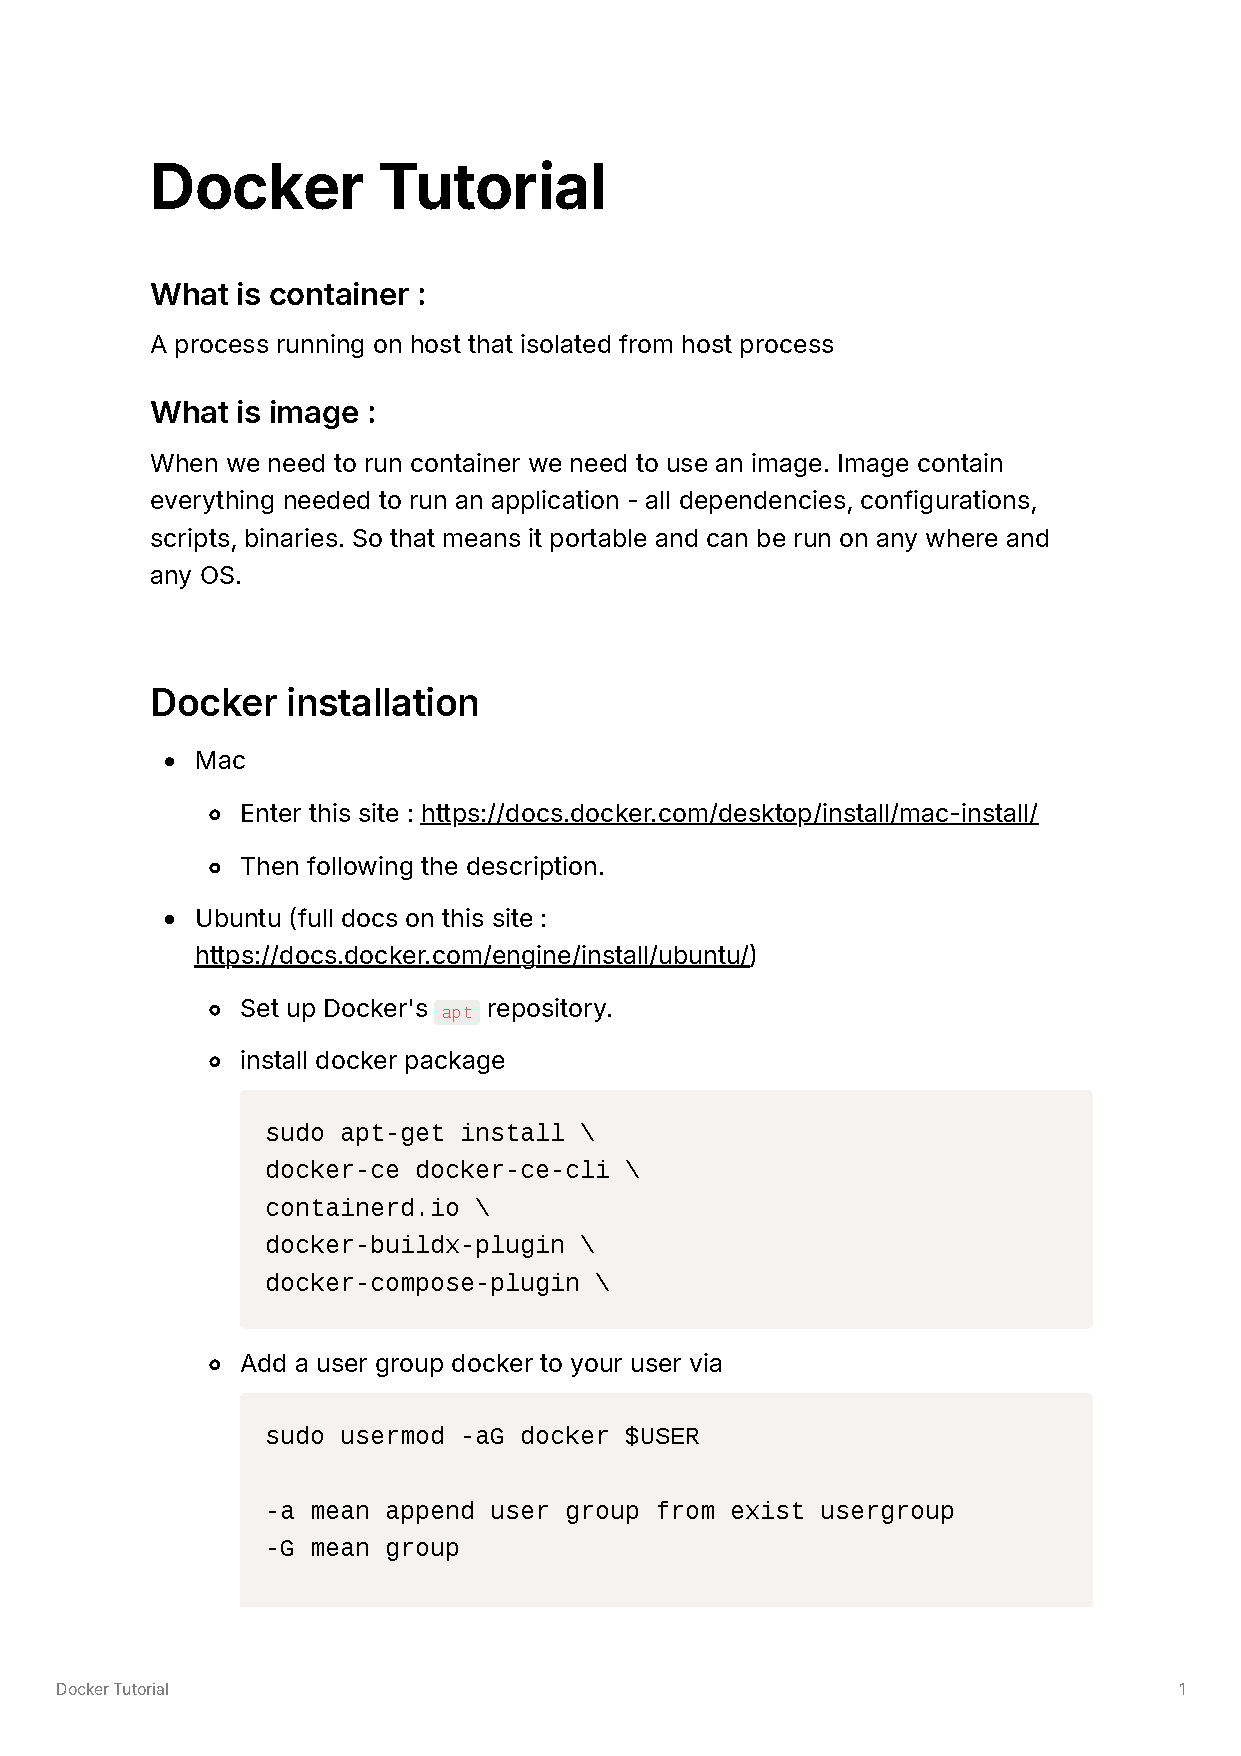
\includepdf[pages=-, scale=.8, pagecommand={\hypertarget{target:docker}{},\label{page:docker}}, nup=1x1, frame=false]{pdf/docker}
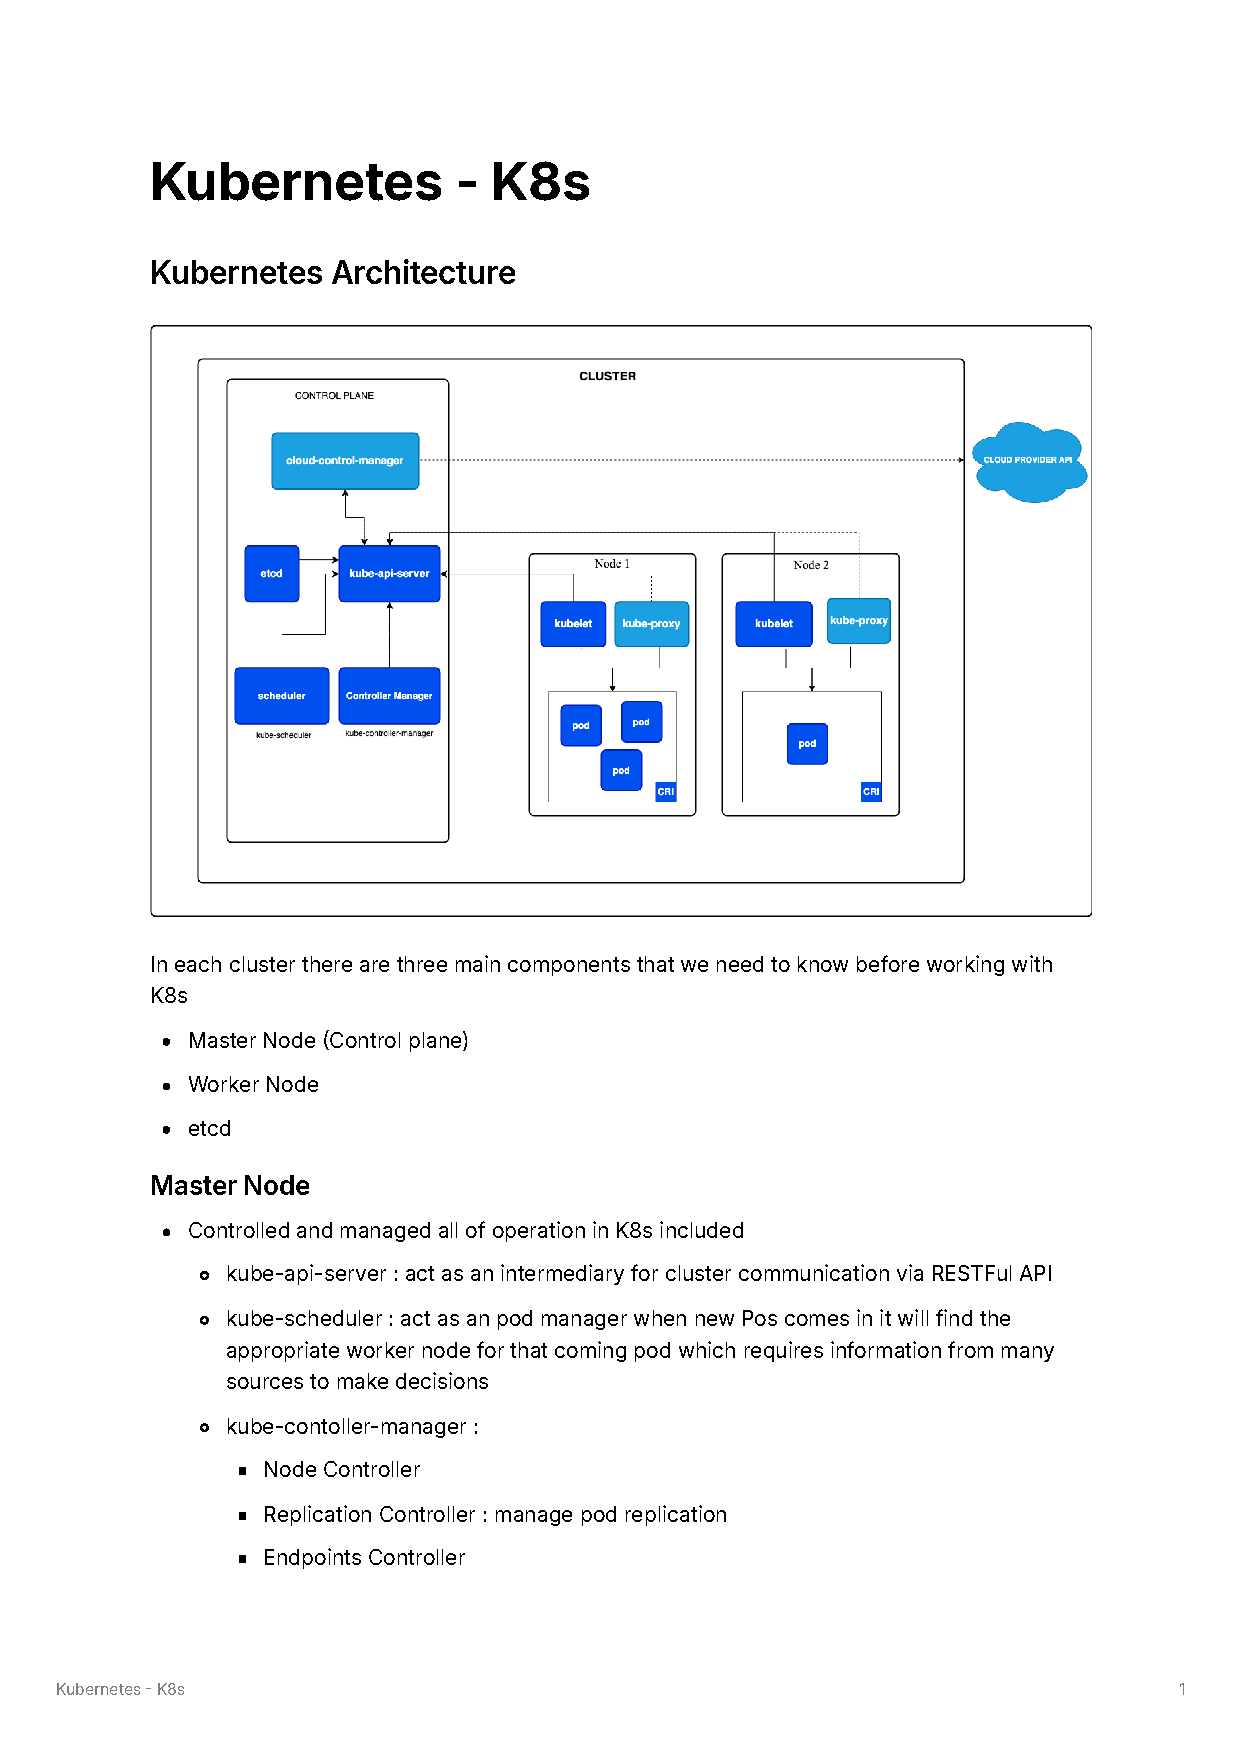
\includepdf[pages=-, scale=.8, pagecommand={\hypertarget{target:kube}{},\label{page:kube}}, nup=1x1, frame=false]{pdf/kube}
\includepdf[pages=-, scale=.8, pagecommand={\hypertarget{target:jenkins}{},\label{page:jenkins}}, nup=1x1, frame=false]{pdf/jenkins}
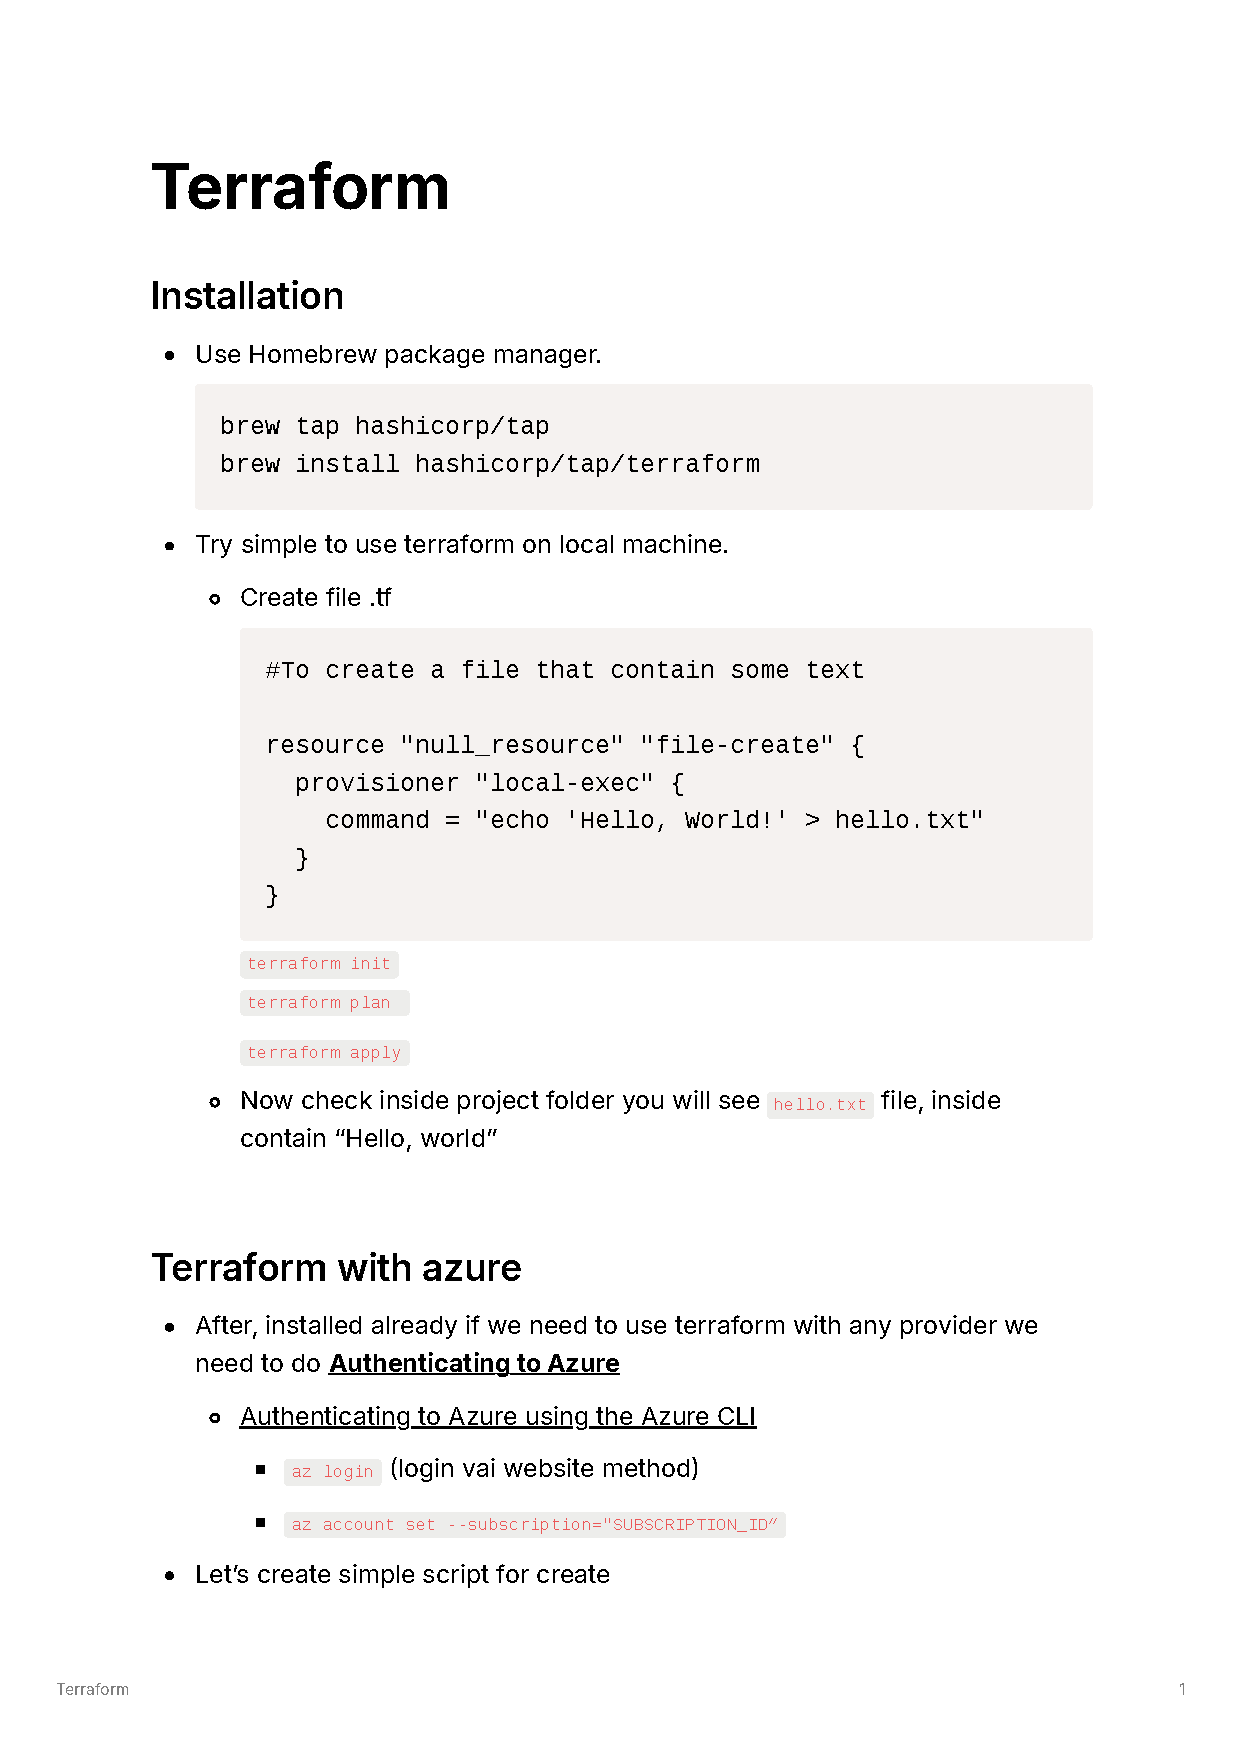
\includepdf[pages=-, scale=.8, pagecommand={\hypertarget{target:terraform}{},\label{page:terraform}}, nup=1x1, frame=false]{pdf/terraform}
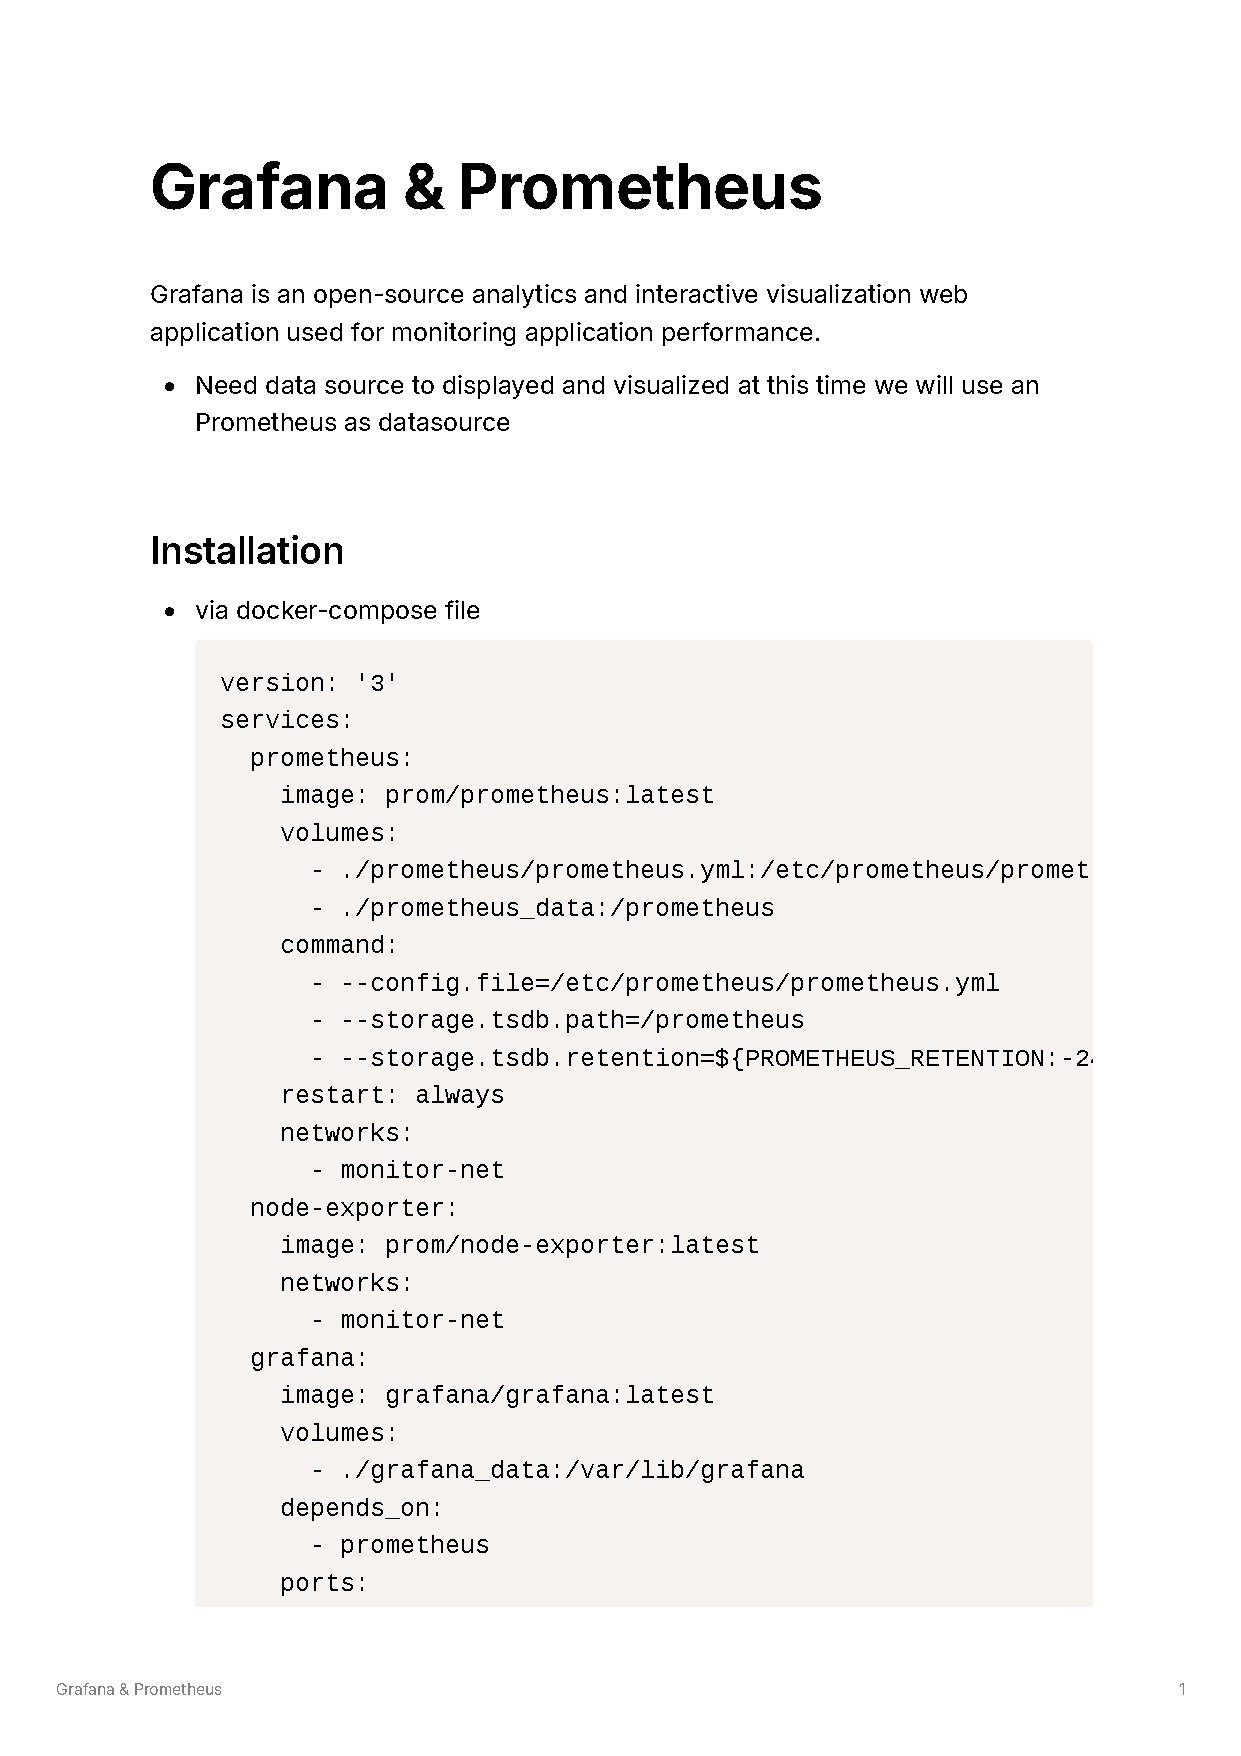
\includepdf[pages=-, scale=.8, pagecommand={\hypertarget{target:monitoring}{},\label{page:monitoring}}, nup=1x1, frame=false]{pdf/monitoring}
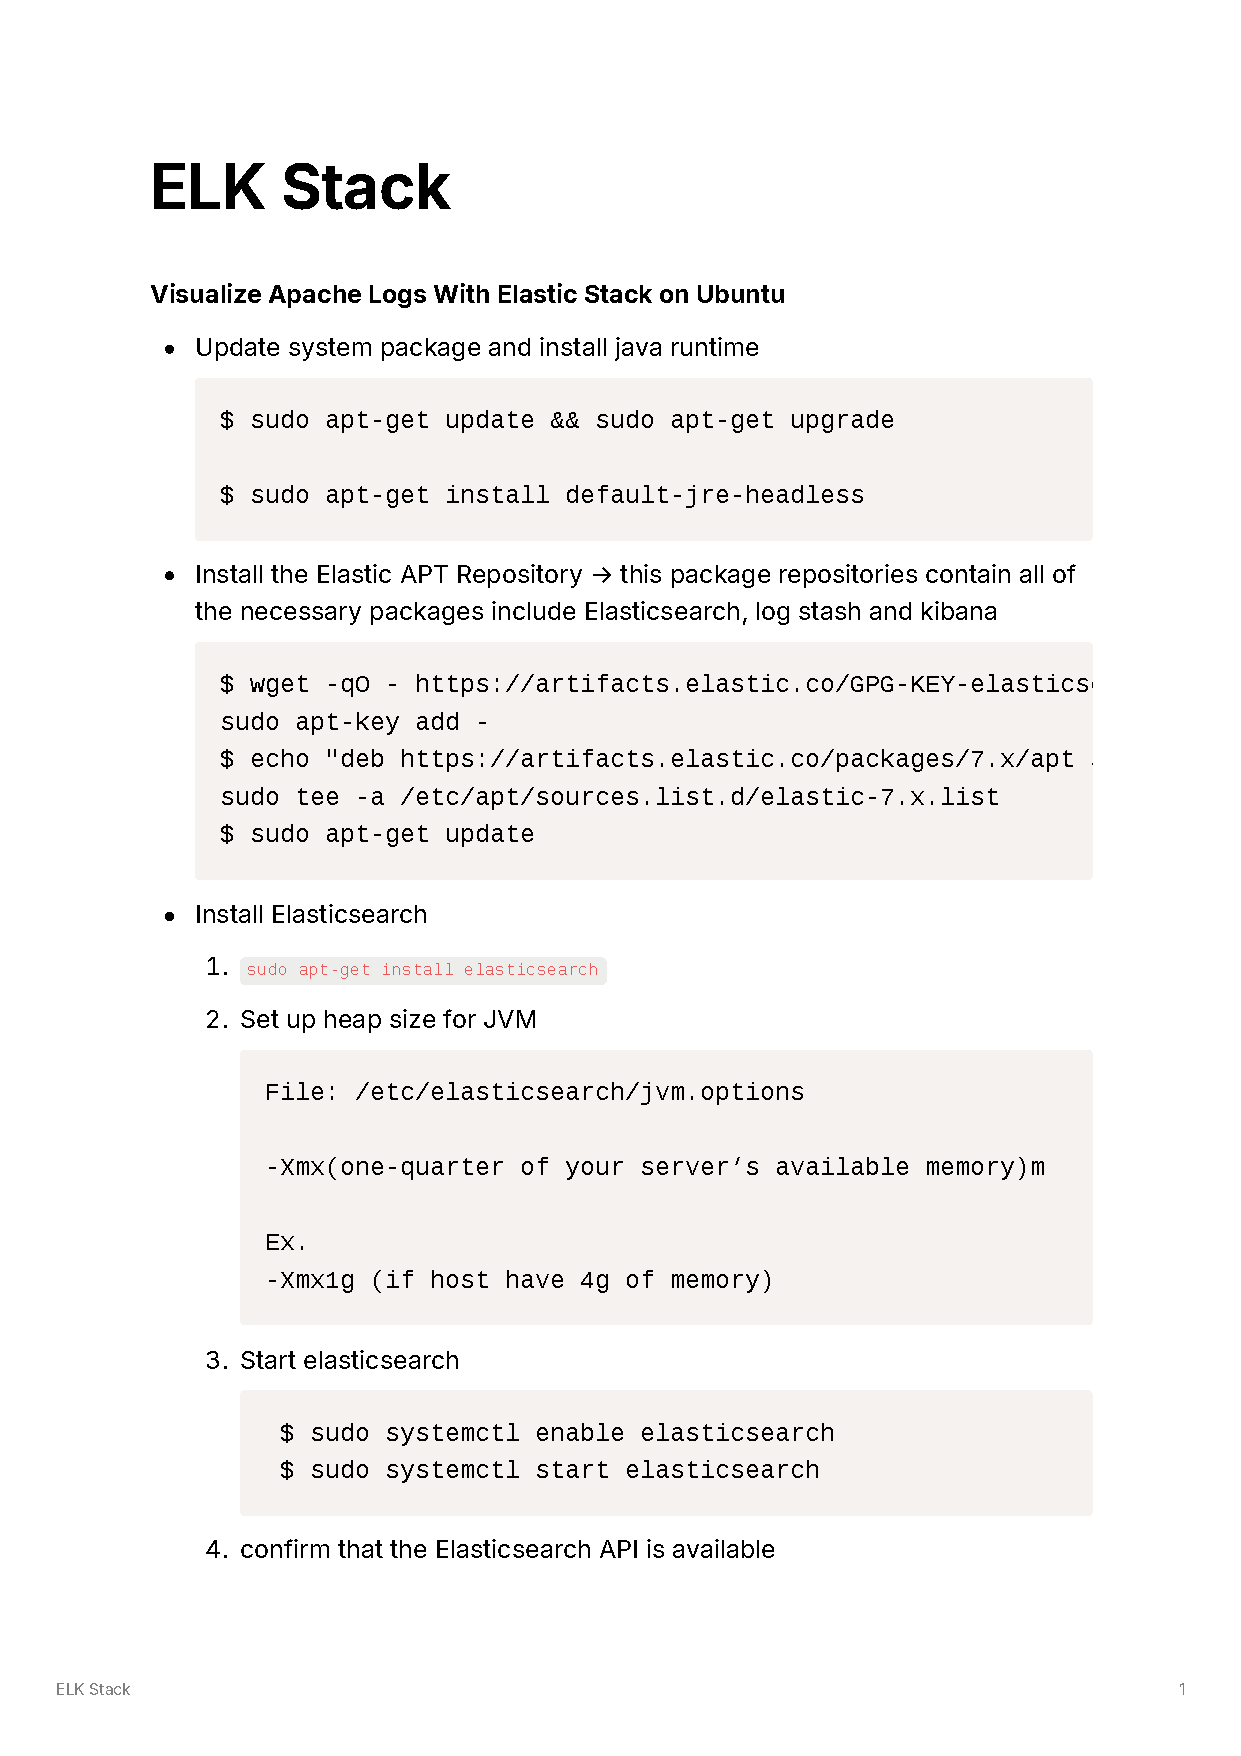
\includepdf[pages=-, scale=.8, pagecommand={\hypertarget{target:elk}{},\label{page:elk}}, nup=1x1, frame=false]{pdf/elk}